% ============================================================================
% MÓDULO 2 — CAPÍTULO 6
% CHF662 — ANÁLISE AMBIENTAL (DCHF/UEFS)
% ============================================================================

\chapter{Fundamentos da Análise Ambiental Integrada, Escalas e Ordenamento Territorial}
\label{cap:analise_integrada}

\noindent\tagEmenta\ \tagPratica
\par\vspace{6pt}

% ============================================================================
% ETAPA 1 — OBJETIVOS
% ============================================================================
\begin{capObjetivos}
  Ao concluir este capítulo, você será capaz de:
  \begin{itemize}[leftmargin=1.5em, itemsep=2.5pt]
    \item Integrar os elementos e fatores dos meios \textbf{físico}, \textbf{biótico} e \textbf{antrópico}, superando inventários setoriais fragmentados na Análise Ambiental.
    \item Diferenciar e acoplar \textbf{escalas espaciais} (parcela, vertente, microbacia, bacia regional e bioma) e \textbf{escalas temporais} (evento, sazonal, histórica e geológica), identificando e evitando a \textbf{falácia de escala}.
    \item Modelar o ambiente como um \textbf{sistema ambiental aberto}, calculando balanços de massa e estoques ($\Delta S = E - S_{\text{out}}$), interpretando limiares (\textit{thresholds}) e distinguindo retroalimentação (\textit{feedback}) positiva de negativa.
    \item Estabelecer a distinção conceitual e operacional rigorosa entre \textbf{planejamento ambiental}, \textbf{planejamento territorial} e \textbf{ordenamento territorial}.
    \item Explicar a estrutura, o marco legal e a aplicação do \textbf{Zoneamento Ecológico-Econômico (ZEE)} como instrumento central de ordenamento territorial.
  \end{itemize}
\end{capObjetivos}

% ============================================================================
% ETAPA 2 — REVISÃO
% ============================================================================
\begin{capRevisao}
  Para aproveitar plenamente este capítulo, resgate três fundamentos trabalhados anteriormente:
  \begin{enumerate}[leftmargin=1.6em, itemsep=2.5pt]
    \item \textbf{Geografia Socioambiental (Cap. 3):} o ambiente é uma totalidade híbrida em que processos naturais e práticas sociais se codeterminam historicamente; analisar relevo ou água sem considerar uso da terra e conflitos territoriais produz diagnósticos incompletos.
    \item \textbf{Resiliência e fragilidade (Cap. 4):} os sistemas ambientais absorvem perturbações até determinado limite; ultrapassado esse patamar, mudam abruptamente de estado funcional.
    \item \textbf{Diagnóstico e áreas de influência na AIA (Cap. 5):} a escolha da escala de análise (ADA, AID, AII) determina quais processos aparecem no mapa e quais desaparecem por generalização cartográfica.
  \end{enumerate}
\end{capRevisao}

% ============================================================================
% ETAPA 3 — EXPLICAÇÃO TEÓRICA
% ============================================================================
\etapa{3}{Explicação Teórica e Fundamentos Metodológicos}

\begin{boxSimbolo}[Vocabulário Sistêmico, Escalar e de Ordenamento]
  \renewcommand{\arraystretch}{1.18}
  \small
  \begin{tabularx}{\textwidth}{@{}l >{\raggedright\arraybackslash}X@{}}
    \toprule
    \textbf{Termo / Símbolo} & \textbf{Definição operacional na Análise Ambiental Integrada} \\
    \midrule
    \textbf{Sistema aberto} & Conjunto de componentes inter-relacionados que troca continuamente matéria e energia com o meio externo por meio de entradas ($E$) e saídas ($S_{\text{out}}$). \\
    \textbf{$\Delta S = E - S_{\text{out}}$} & Equação de balanço de massa ou energia: variação do estoque interno ($\Delta S$) igual à diferença entre entradas e saídas em determinado intervalo de tempo. \\
    \textbf{Limiar (\textit{Threshold})} & Valor crítico de uma variável a partir do qual o sistema altera abruptamente seu regime de funcionamento (por exemplo, intensidade de chuva superior à capacidade de infiltração do solo). \\
    \textbf{Retroalimentação} & Mecanismo de retorno pelo qual uma saída influencia novas entradas ou processos internos; pode ser \textbf{negativa} (estabilizadora) ou \textbf{positiva} (amplificadora de mudança/degradação). \\
    \textbf{Falácia de escala} & Erro metodológico de extrapolar diretamente taxas, relações causais ou padrões observados em uma escala espacial ou temporal para outra escala sem considerar os processos emergentes intermediários. \\
    \textbf{SDR ($Y / E_b$)} & Razão de Entrega de Sedimentos (\textit{Sediment Delivery Ratio}): fração da erosão bruta das vertentes ($E_b$) que efetivamente alcança o exutório da bacia ($Y$). \\
    \textbf{ZEE} & Zoneamento Ecológico-Econômico: instrumento de ordenamento territorial que integra potencialidades e fragilidades geoambientais e socioeconômicas em zonas com diretrizes de uso. \\
    \bottomrule
  \end{tabularx}
\end{boxSimbolo}

\section{Elementos dos Meios Físico, Biótico e Antrópico e suas Interações}

Um erro recorrente em relatórios ambientais consiste em tratar o diagnóstico como uma colagem de capítulos isolados sobre rochas, plantas e população, sem explicar como esses compartimentos interagem na paisagem. A \textbf{Análise Ambiental Integrada} (Castro; Lemos, 2016; Drew, 1989) rompe com essa visão compartimentada ao focar tanto os \emph{elementos} constituintes quanto, sobretudo, as \textbf{relações funcionais} que conectam os três subsistemas da paisagem.

O \textbf{meio físico (abiótico)} abrange o substrato geológico, as formas de relevo e declividade, os tipos e propriedades dos solos, o regime climático (chuva, radiação e evapotranspiração) e a dinâmica hidrológica superficial e subterrânea, fornecendo a matriz energética, topográfica e material de suporte do sistema. Sobre essa base atua o \textbf{meio biótico}, composto pelas formações vegetais, fauna, microrganismos edáficos, teias tróficas e fluxos gênicos, que funciona como regulador ativo do meio físico ao interceptar gotas de chuva, elevar a rugosidade superficial, estruturar o solo com matéria orgânica e raízes e reciclar nutrientes. Por sua vez, o \textbf{meio antrópico (socioeconômico e cultural)} reúne os padrões de uso e cobertura da terra, os sistemas agropecuários, a urbanização, a infraestrutura viária e energética, a estrutura fundiária, a organização comunitária e as instituições públicas, operando simultaneamente como agente transformador dos fluxos de matéria e energia e como receptor das alterações ambientais desencadeadas.

No Semiárido baiano, essas interações tornam-se imediatamente visíveis em uma única encosta de Caatinga. A retirada da vegetação lenhosa (ação antrópica sobre o meio biótico) expõe um Neossolo ou Argissolo raso (meio físico) ao impacto direto das chuvas torrenciais convectivas, reduz a matéria orgânica e a infiltração, acelera o escoamento superficial, abre sulcos e ravinas, assoreia o barreiro ou açude comunitário e agrava a escassez de água na estiagem, gerando um retorno direto sobre o meio socioeconômico.

\section{Sistemas Ambientais Abertos, Limiares e Retroalimentação}

A fundamentação sistêmica da Análise Ambiental apoia-se na Teoria Geral dos Sistemas (Bertalanffy, 2010) e na abordagem dos sistemas ambientais (Drew, 1989; Christofoletti, 1999). Paisagens, vertentes e bacias hidrográficas são \textbf{sistemas ambientais abertos}, isto é, recebem continuamente fluxos externos de matéria e energia (\textbf{entradas} ou \textit{inputs}, como radiação solar, chuva, insumos agrícolas e trabalho humano), transformam e armazenam parte desses fluxos em \textbf{estoques internos} (solo, água subterrânea, biomassa, nutrientes) por meio de \textbf{processos} (infiltração, intemperismo, fotossíntese, erosão) e exportam fluxos (\textbf{saídas} ou \textit{outputs}, como vazão fluvial, sedimentos, evapotranspiração e colheitas).

O Painel A da Figura~\ref{fig:sistema_escalas} ilustra essa arquitetura aberta e o circuito de retorno (\textbf{retroalimentação} ou \textit{feedback}), que governa a estabilidade ou o colapso do sistema.

\begin{figure}[htbp]
  \centering
  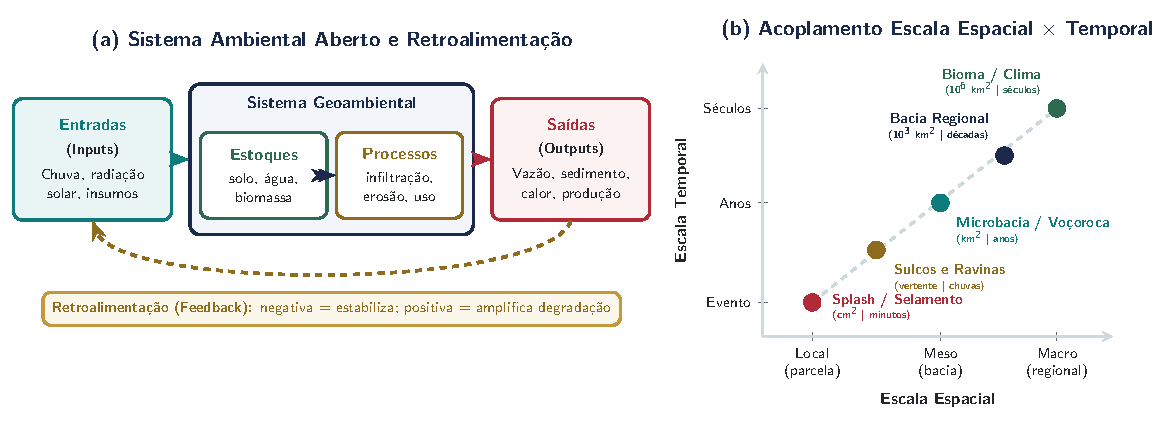
\includegraphics[width=0.95\textwidth]{figures/fig04_sistema_aberto_escalas.pdf}
  \caption{Representação do sistema ambiental aberto com entradas, estoques, processos, saídas e retroalimentação (Painel A) e acoplamento entre escalas espaciais e temporais na dinâmica geoambiental (Painel B). Fonte: elaboração didática da disciplina CHF662 com base em Drew (1989) e Castro; Lemos (2016).}
  \label{fig:sistema_escalas}
\end{figure}

\begin{boxConceito}[Equilíbrio Dinâmico, Limiares (\textit{Thresholds}) e Retroalimentação]
  Em um sistema ambiental aberto, o \textbf{equilíbrio dinâmico (\textit{steady state})} ocorre quando as entradas e saídas se compensam em média ao longo do tempo ($\Delta S \approx 0$), mantendo os estoques estáveis apesar da circulação contínua de água, energia e matéria; trata-se de autorregulação ativa, e não de imobilidade. Essa estabilidade depende da \textbf{retroalimentação negativa (\textit{feedback} negativo)}, mecanismo estabilizador que amortece uma perturbação e devolve o sistema ao estado de referência. Em uma vertente bem vegetada, por exemplo, um aumento moderado de chuva eleva a umidade do solo, estimula o crescimento herbáceo, amplia a interceptação e a infiltração e, por consequência, reduz o escoamento erosivo.

  Em sentido oposto, a \textbf{retroalimentação positiva (\textit{feedback} positivo)} atua como mecanismo amplificador que reforça o desvio inicial, podendo conduzir o sistema à degradação acelerada. Na dinâmica de desertificação ou erosão linear, o sobrepastejo reduz a cobertura vegetal, o que aumenta o selamento e a compactação do solo, derruba a infiltração e eleva o escoamento superficial; essa enxurrada carreia matéria orgânica e sementes, dificulta ainda mais a regeneração vegetal e acelera a abertura de ravinas e voçorocas. Essa transição de regime ocorre quando se ultrapassam \textbf{limiares (\textit{thresholds})}, definidos como pontos críticos de ruptura a partir dos quais o sistema muda de comportamento. Tais limiares podem ser \textbf{extrínsecos}, quando disparados por um evento externo (como uma chuva cuja intensidade ultrapassa a taxa máxima de infiltração do solo, $I > f_c$), ou \textbf{intrínsecos}, quando resultam do enfraquecimento interno gradual do próprio sistema (como o desgaste progressivo da coesão de um talude até o rompimento repentino).
\end{boxConceito}

\section{Escalas Espaciais, Escalas Temporais e o Risco da Falácia de Escala}

Nenhum processo geoambiental ocorre fora de uma escala determinada. Como mostra o Painel B da Figura~\ref{fig:sistema_escalas}, existe um \textbf{acoplamento natural entre escala espacial e escala temporal}: processos microscópicos ou pontuais costumam ocorrer em minutos ou horas, enquanto transformações de bacias regionais e biomas desdobram-se em décadas, séculos ou milênios.

\begin{center}
\renewcommand{\arraystretch}{1.20}
\small
\begin{tabularx}{\textwidth}{@{}p{2.7cm} p{2.5cm} p{2.7cm} >{\raggedright\arraybackslash}X@{}}
  \toprule
  \rowcolor{uefsNavy}
  \textcolor{white}{\bfseries Escala Espacial} & \textcolor{white}{\bfseries Ordem de Área} & \textcolor{white}{\bfseries Escala Temporal Típica} & \textcolor{white}{\bfseries Processos e Aplicações Dominantes} \\
  \midrule
  \textbf{Parcela / Microescala} & $\text{cm}^2$ a $10^2\,\text{m}^2$ & Minutos a horas (evento chuvoso) & Impacto da gota (\textit{splash}), selamento superficial, infiltração pontual e erosão laminar inicial. \\
  \rowcolor{bgGray}
  \textbf{Vertente / Encosta} & $10^2\,\text{m}^2$ a $\text{ha}$ & Chuvas intensas a ciclos sazonais & Escoamento concentrado, formação de sulcos e ravinas, deslizamentos de taludes e manejo conservacionista local. \\
  \textbf{Microbacia} & $1$ a $50\,\text{km}^2$ & Meses a anos (ciclos anuais) & Evolução de voçorocas, conectividade vertente--canal, balanço hídrico local, PRAD e diagnósticos municipais. \\
  \rowcolor{bgGray}
  \textbf{Bacia Regional} & $10^2$ a $10^5\,\text{km}^2$ & Anos a décadas (escala histórica) & Assoreamento de grandes reservatórios, conflitos pelo uso da água, planos de bacia e ZEE estadual. \\
  \textbf{Bioma / Macroescala} & $> 10^5\,\text{km}^2$ & Décadas a milênios (tempo geológico/climático) & Dinâmica climática regional, aridização/desertificação, evolução geomorfológica e grandes políticas territoriais. \\
  \bottomrule
\end{tabularx}
\end{center}

Ignorar o acoplamento entre escalas leva à \textbf{falácia de escala}, um dos erros mais graves na Geografia e na Análise Ambiental, que se manifesta em duas direções opostas. Na \textbf{extrapolação ascendente indevida (micro para macro)}, assume-se que uma taxa de erosão medida em parcela experimental de $10\,\text{m}^2$ multiplica-se linearmente por toda uma bacia de $1\,000\,\text{ha}$; na realidade, grande parte do solo erodido nas encostas fica retida em sopés côncavos, depressões, barreiras vegetais e planícies aluviais antes de atingir o rio principal, fazendo com que a Razão de Entrega de Sedimentos (SDR) seja inferior à unidade. Na \textbf{inferência descendente indevida (macro para micro)}, utiliza-se um mapa de escala pequena ($1:250\,000$ ou $1:1\,000\,000$), elaborado para planejamento estadual, para localizar uma ravina de $4\,\text{m}$ de largura ou projetar uma paliçada de bioengenharia. Em escala cartográfica $1:D$, o menor detalhe graficamente distinguível no papel ($\approx 0{,}2\,\text{mm} = 0{,}0002\,\text{m}$) corresponde no terreno a $d_{\min} = 0{,}0002 \times D$ metros; logo, em uma carta $1:250\,000$, qualquer feição menor que $50\,\text{m}$ desaparece da representação gráfica.

\begin{boxFormula}[Balanço de Massa em Sistema Aberto, Razão de Entrega de Sedimentos (SDR) e Resolução de Escala]
  \textbf{1. Equação geral do balanço em um sistema ambiental aberto:}
  \[
    \Delta S = E - S_{\text{out}}
  \]
  Para o \textbf{balanço hídrico} de uma microbacia (em $\text{mm/ano}$):
  \[
    \Delta S = P - \left(ET + Q_s + Q_b\right)
  \]
  onde $P$ é a precipitação (entrada), $ET$ é a evapotranspiração real, $Q_s$ é o escoamento superficial direto e $Q_b$ é o escoamento de base/drenagem profunda (saídas). Se $\Delta S = 0$, há equilíbrio dinâmico; se $\Delta S < 0$, ocorre depleção do estoque hídrico do solo/aquífero; se $\Delta S > 0$, ocorre recarga.

  \vspace{4pt}
  \textbf{2. Razão de Entrega de Sedimentos (\textit{Sediment Delivery Ratio}, SDR) e quantificação da falácia de escala:}
  \[
    \text{SDR} = \frac{Y}{E_b} \qquad \Longleftrightarrow \qquad Y = E_b \times \text{SDR}, \qquad \text{com } 0 < \text{SDR} \le 1
  \]
  onde $E_b$ é a erosão bruta nas vertentes ($\text{t/(ha}\cdot\text{ano)}$) e $Y$ é a produção específica de sedimentos medida no exutório da bacia ($\text{t/(ha}\cdot\text{ano)}$). Para uma bacia de área $A$ ($\text{ha}$), sendo $E_{b,\text{tot}} = E_b \times A$ a erosão bruta total e $Y_{\text{tot}} = Y \times A$ o aporte total no exutório ($\text{t/ano}$), a massa total retida internamente nas encostas e planícies (colúvios e alúvios) é $R_{\text{sed}} = (E_b - Y) \times A$. Quando um analista extrapola dados de parcela para a bacia assumindo implicitamente $\text{SDR} = 1$, comete erro relativo de superestimativa igual a:
  \[
    \text{Erro (\%)} = \frac{E_{b,\text{tot}} - Y_{\text{tot}}}{Y_{\text{tot}}} \times 100\% = \left(\frac{1}{\text{SDR}} - 1\right) \times 100\%.
  \]

  \vspace{4pt}
  \textbf{3. Menor feição representável em carta de escala $1:D$ (erro gráfico de $0{,}2\,\text{mm}$):}
  \[
    d_{\min}\,(\text{m}) = 0{,}0002 \times D.
  \]
\end{boxFormula}

\section{Dinâmica Geoambiental, Planejamento Ambiental, Planejamento Territorial e Ordenamento Territorial}

Compreender a \textbf{dinâmica geoambiental}, isto é, o comportamento integrado das paisagens frente às pressões climáticas e socioeconômicas, é a base técnica indispensável para orientar decisões públicas sobre o uso do espaço. Contudo, na literatura técnica e em concursos, três expressões correlatas são frequentemente confundidas: \textbf{planejamento ambiental}, \textbf{planejamento territorial} e \textbf{ordenamento territorial} (Arruda, 2013; IBGE, 2018).

\begin{center}
\renewcommand{\arraystretch}{1.22}
\small
\begin{tabularx}{\textwidth}{@{}p{2.9cm} >{\raggedright\arraybackslash}X >{\raggedright\arraybackslash}X p{3.1cm}@{}}
  \toprule
  \rowcolor{uefsNavy}
  \textcolor{white}{\bfseries Conceito} & \textcolor{white}{\bfseries Objeto e foco central} & \textcolor{white}{\bfseries Natureza e função} & \textcolor{white}{\bfseries Instrumentos típicos} \\
  \midrule
  \textbf{Planejamento Ambiental} & Qualidade dos ecossistemas, recursos naturais, fragilidades, riscos e serviços ecossistêmicos. & Processo contínuo de diagnóstico, prognóstico e formulação de diretrizes para conservar, recuperar e compatibilizar atividades humanas à capacidade de suporte ambiental. & AIA, Planos de Bacia Hidrográfica, Planos de Manejo de UCs, PRAD, planos municipais de saneamento e conservação. \\
  \rowcolor{bgGray}
  \textbf{Planejamento Territorial} & Organização socioespacial abrangente (economia, infraestrutura, mobilidade, habitação, redes urbanas e rurais, incluindo a dimensão ambiental). & Processo estratégico multissetorial de definição de cenários, prioridades de investimento e articulação de políticas públicas sobre o território. & Planos Diretores Municipais, Planos de Desenvolvimento Regional, Planos Plurianuais territorializados. \\
  \textbf{Ordenamento Territorial} & Regulação espacial efetiva da distribuição das atividades, usos do solo e ocupação humana no território. & Expressão \textbf{normativa, cartográfica e vinculante} do Estado para compatibilizar usos produtivos, infraestrutura e proteção ambiental, reduzindo conflitos socioespaciais. & \textbf{Zoneamento Ecológico-Econômico (ZEE)}, macrozoneamento do Plano Diretor, zoneamento costeiro e agrícola. \\
  \bottomrule
\end{tabularx}
\end{center}

Em síntese operacional, o \textbf{planejamento ambiental} define os limites, potenciais e fragilidades dos sistemas naturais; o \textbf{planejamento territorial} integra esses condicionantes às demandas econômicas, sociais e de infraestrutura; e o \textbf{ordenamento territorial} traduz essas diretrizes em normas espaciais e zoneamentos concretos de regulação do uso da terra.

\section{Zoneamento Ecológico-Econômico (ZEE) como Instrumento de Ordenamento}

Previsto originalmente na Política Nacional do Meio Ambiente (Lei nº 6.938/1981) e regulamentado pelo \textbf{Decreto Federal nº 4.297/2002}, o \textbf{Zoneamento Ecológico-Econômico (ZEE)} é o principal instrumento técnico-político de organização do território no Brasil. Longe de constituir um conjunto estático de restrições ou um documento meramente cartográfico, o ZEE opera como um processo participativo e multidisciplinar que cruza a \textbf{potencialidade socioeconômica} com a \textbf{vulnerabilidade e fragilidade natural} dos sistemas geoambientais (IBGE, 2018; Arruda, 2013).

A partir desse cruzamento, o território é dividido em \textbf{zonas homogêneas} com regras específicas de uso, manejo e investimento público. As \textbf{Zonas de Consolidação Produtiva} reúnem áreas de alta aptidão e baixa fragilidade natural, nas quais o uso agropecuário, industrial ou urbano deve ser otimizado com boas práticas de conservação de solo e água. Já as \textbf{Zonas de Uso Restrito ou Manejo Sustentável} correspondem a áreas de fragilidade média a alta que admitem atividades produtivas de baixo impacto, como extrativismo sustentável, sistemas agroflorestais, ecoturismo e manejo da Caatinga. Em áreas já submetidas a processos de degradação (erosão acelerada, desertificação e matas ciliares suprimidas), instituem-se \textbf{Zonas de Recuperação Ambiental}, prioritárias para PRAD, bioengenharia e recomposição florestal. Por sua vez, as \textbf{Zonas de Proteção e Conservação} abrangem setores de altíssima fragilidade, relevância hídrica ou biodiversidade endêmica (APPs, nascentes, Unidades de Conservação e corredores ecológicos), voltados prioritariamente à preservação.

O ZEE dialoga diretamente com a AIA (Capítulo 5), pois, quando um estado ou município dispõe de um ZEE atualizado em escala compatível, a etapa de triagem e a seleção de alternativas locacionais tornam-se muito mais céleres, transparentes e seguras juridicamente.

% ============================================================================
% ETAPA 4 — ESTUDOS DE CASO E EXEMPLOS RESOLVIDOS (5 EXEMPLOS, 7 PASSOS CADA)
% ============================================================================
\etapa{4}{Estudos de Caso e Exemplos Resolvidos Passo a Passo}

\begin{boxExemplo}{6.1}{Balanço Hídrico em Sistema Ambiental Aberto no Semiárido (Nível Básico)}
  \passoEnunciado{Uma microbacia experimental inserida no domínio da Caatinga foi monitorada durante um ano hidrológico completo. Deseja-se avaliar se o sistema hídrico local operou em equilíbrio dinâmico, recarga ou depleção de estoque.}
  \passoDados{Entrada anual de precipitação $P = 680\,\text{mm/ano}$. Saídas anuais medidas: evapotranspiração real $ET = 545\,\text{mm/ano}$; escoamento superficial direto $Q_s = 115\,\text{mm/ano}$; escoamento de base / drenagem profunda $Q_b = 35\,\text{mm/ano}$.}
  \passoPedido{Calcular o total de saídas ($S_{\text{out}}$), a variação do estoque hídrico interno ($\Delta S$) e interpretar o estado funcional do sistema nesse ano hidrológico.}
  \passoMetodo{Aplicação da equação de conservação de massa em sistema ambiental aberto: $\Delta S = P - (ET + Q_s + Q_b)$.}
  \passoContas{%
    \begin{enumerate}[leftmargin=1.5em, itemsep=2pt]
      \item \textbf{Soma das saídas do sistema ($S_{\text{out}}$):}
      \[
        S_{\text{out}} = ET + Q_s + Q_b = 545 + 115 + 35 = 695\,\text{mm/ano}.
      \]
      \item \textbf{Variação do estoque hídrico ($\Delta S$):}
      \[
        \Delta S = P - S_{\text{out}} = 680 - 695 = -15\,\text{mm/ano}.
      \]
      \item \textbf{Interpretação física:} o sinal negativo ($\Delta S = -15\,\text{mm/ano}$) indica que as saídas superaram as entradas em $15\,\text{mm}$; logo, o sistema consumiu parte da água armazenada previamente no solo e nos reservatórios subterrâneos rasos (depleção líquida de estoque).
    \end{enumerate}
  }
  \passoResposta{Total de saídas $S_{\text{out}} = 695\,\text{mm/ano}$ e variação do estoque $\Delta S = -15\,\text{mm/ano}$, caracterizando depleção moderada do estoque hídrico interno nesse ano.}
  \passoVerificacao{O valor é fisicamente coerente para o Semiárido baiano: a evapotranspiração consome a maior parcela da chuva ($545/680 \approx 80{,}15\%$), e déficits interanuais moderados de estoque são esperados em anos de precipitação ligeiramente abaixo da média, sendo compensados nos anos mais chuvosos se a cobertura vegetal preservar a infiltração.}
\end{boxExemplo}

\begin{boxExemplo}{6.2}{Quantificando a Falácia de Escala pela Razão de Entrega de Sedimentos: SDR (Nível Básico–Intermediário)}
  \passoEnunciado{Em uma parcela experimental de $20\,\text{m}^2$ de solo exposto em uma microbacia do Piemonte da Diamantina, mediu-se uma taxa de erosão bruta de $E_b = 24{,}0\,\text{t/(ha}\cdot\text{ano)}$. Para estimar o assoreamento de um açude no exutório da bacia (área total $A = 1\,500\,\text{ha}$), um técnico multiplicou diretamente a taxa da parcela pela área da bacia. Entretanto, o monitoramento hidrossedimentológico no exutório registrou uma chegada efetiva de $Y_{\text{tot}} = 9\,720\,\text{t/ano}$.}
  \passoDados{$E_b = 24{,}0\,\text{t/(ha}\cdot\text{ano)}$; área da bacia $A = 1\,500\,\text{ha}$; produção total medida no exutório $Y_{\text{tot}} = 9\,720\,\text{t/ano}$.}
  \passoPedido{Calcular: (a) a erosão bruta total estimada pela extrapolação linear do técnico; (b) a produção específica real $Y$; (c) a Razão de Entrega de Sedimentos (SDR); (d) a massa anual de sedimentos retida nas vertentes e planícies; e (e) o erro percentual causado pela falácia de escala.}
  \passoMetodo{Aplicação das relações de escala hidrossedimentológica: $E_{b,\text{tot}} = E_b \cdot A$, $Y = Y_{\text{tot}}/A$, $\text{SDR} = Y / E_b$, $R_{\text{sed}} = E_{b,\text{tot}} - Y_{\text{tot}}$ e $\text{Erro (\%)} = (E_{b,\text{tot}} - Y_{\text{tot}})/Y_{\text{tot}} \times 100\%$.}
  \passoContas{%
    \begin{enumerate}[leftmargin=1.5em, itemsep=2pt]
      \item \textbf{Extrapolação linear do técnico (erosão bruta total):}
      \[
        E_{b,\text{tot}} = 24{,}0\,\text{t/(ha}\cdot\text{ano)} \times 1\,500\,\text{ha} = 36\,000\,\text{t/ano}.
      \]
      \item \textbf{Produção específica real de sedimentos no exutório ($Y$):}
      \[
        Y = \frac{9\,720\,\text{t/ano}}{1\,500\,\text{ha}} = 6{,}48\,\text{t/(ha}\cdot\text{ano)}.
      \]
      \item \textbf{Razão de Entrega de Sedimentos (SDR):}
      \[
        \text{SDR} = \frac{Y}{E_b} = \frac{6{,}48}{24{,}0} = 0{,}27 \quad (\text{ou } 27\%).
      \]
      \item \textbf{Massa de sedimentos retida internamente na bacia:}
      \[
        R_{\text{sed}} = 36\,000 - 9\,720 = 26\,280\,\text{t/ano} \quad (73\% \text{ do solo mobilizado}).
      \]
      \item \textbf{Erro percentual de superestimativa (falácia de escala):}
      \[
        \text{Erro (\%)} = \frac{36\,000 - 9\,720}{9\,720} \times 100\% = \frac{26\,280}{9\,720} \times 100\% \approx 270{,}37\%.
      \]
    \end{enumerate}
  }
  \passoResposta{$E_{b,\text{tot}} = 36\,000\,\text{t/ano}$; $Y = 6{,}48\,\text{t/(ha}\cdot\text{ano)}$; $\text{SDR} = 0{,}27$; sedimentos retidos $= 26\,280\,\text{t/ano}$; erro de superestimativa $= 270{,}37\%$.}
  \passoVerificacao{Confere-se a fórmula alternativa do erro: $(1/\text{SDR} - 1)\times 100\% = (1/0{,}27 - 1)\times 100\% = (3{,}7037 - 1)\times 100\% = 270{,}37\%$. Ambientalmente, esse resultado demonstra a essência da \textbf{falácia de escala}: taxas medidas em parcela de $20\,\text{m}^2$ não consideram a rede de deposição em sopés, depressões e matas ciliares que retém $73\%$ dos sedimentos ao longo de uma bacia de $1\,500\,\text{ha}$.}
\end{boxExemplo}

\begin{boxExemplo}{6.3}{Limiar de Infiltração e Retroalimentação Positiva versus Negativa (Nível Intermediário)}
  \passoEnunciado{Duas vertentes vizinhas com mesma litologia e declividade no Semiárido baiano recebem a mesma chuva convectiva intensa de $I = 65{,}0\,\text{mm/h}$ durante $1$ hora. A \textbf{Vertente 1} possui cobertura de Caatinga conservada com serrapilheira e capacidade de infiltração estável $f_{c1} = 78{,}0\,\text{mm/h}$. A \textbf{Vertente 2} foi submetida a sobrepastejo contínuo, apresentando solo compactado com capacidade de infiltração reduzida para $f_{c2} = 22{,}0\,\text{mm/h}$.}
  \passoDados{Intensidade da chuva $I = 65{,}0\,\text{mm/h}$; limiar de infiltração da Vertente 1: $f_{c1} = 78{,}0\,\text{mm/h}$; limiar de infiltração da Vertente 2: $f_{c2} = 22{,}0\,\text{mm/h}$.}
  \passoPedido{Calcular o excesso de precipitação transformado em escoamento superficial ($R = \max(0, I - f_c)$) e o percentual da chuva que escoa superficialmente em cada vertente, identificando em qual delas o limiar extrínseco foi rompido e qual tipo de retroalimentação predomina.}
  \passoMetodo{Comparação direta entre a entrada externa ($I$) e o limiar interno de infiltração ($f_c$), seguida da análise sistêmica dos circuitos de retroalimentação.}
  \passoContas{%
    \begin{enumerate}[leftmargin=1.5em, itemsep=2pt]
      \item \textbf{Vertente 1 (Caatinga conservada):}
      Como $I = 65{,}0\,\text{mm/h} < f_{c1} = 78{,}0\,\text{mm/h}$, o limiar de infiltração \textbf{não é ultrapassado}:
      \[
        R_1 = \max(0,\; 65{,}0 - 78{,}0) = 0{,}0\,\text{mm/h} \quad (0\% \text{ de escoamento hortoniano}).
      \]
      Toda a lâmina de $65{,}0\,\text{mm}$ infiltra-se, recarregando a umidade do solo, sustentando a vegetação e mantendo a estrutura porosa (\textbf{retroalimentação negativa}, estabilizadora).
      \item \textbf{Vertente 2 (Pastagem compactada):}
      Como $I = 65{,}0\,\text{mm/h} > f_{c2} = 22{,}0\,\text{mm/h}$, o limiar de infiltração é \textbf{rompido}:
      \[
        R_2 = 65{,}0 - 22{,}0 = 43{,}0\,\text{mm/h}.
      \]
      \item \textbf{Percentual da chuva convertido em escoamento superficial na Vertente 2:}
      \[
        \frac{R_2}{I} \times 100\% = \frac{43{,}0}{65{,}0} \times 100\% \approx 66{,}15\%.
      \]
      Mais de dois terços da chuva escoam velozmente pela superfície, removendo solo fértil, sementes e nutrientes, o que dificulta a regeneração vegetal e reduz ainda mais $f_c$ nas chuvas seguintes (\textbf{retroalimentação positiva}, amplificadora da degradação).
    \end{enumerate}
  }
  \passoResposta{Vertente 1: $R_1 = 0{,}0\,\text{mm/h}$ ($0\%$, abaixo do limiar, retroalimentação negativa). Vertente 2: $R_2 = 43{,}0\,\text{mm/h}$ ($66{,}15\%$ da chuva vira enxurrada, limiar rompido, retroalimentação positiva degradativa).}
  \passoVerificacao{O contraste entre $0\,\text{mm/h}$ e $43{,}0\,\text{mm/h}$ sob exatamente a mesma chuva demonstra que a degradação no Semiárido não decorre apenas da ``força da natureza'', mas da interação entre o evento climático (meio físico) e o manejo do solo/vegetação (meios biótico e antrópico).}
\end{boxExemplo}

\begin{boxExemplo}{6.4}{Escolha de Escala Cartográfica e Erro Gráfico Mínimo em Diagnósticos (Nível Intermediário–Avançado)}
  \passoEnunciado{Uma equipe de Geografia precisa mapear ravinas com largura média de $4{,}0\,\text{m}$ e faixas de mata ciliar de $15{,}0\,\text{m}$ em uma microbacia de $850\,\text{ha}$ ($8{,}5\,\text{km}^2$) próxima a Feira de Santana. A prefeitura dispõe de três bases cartográficas: uma carta regional do ZEE ($1:250\,000$), uma carta topográfica sistemática ($1:50\,000$) e um ortomosaico detalhado ($1:10\,000$).}
  \passoDados{Erro gráfico mínimo no papel $= 0{,}2\,\text{mm} = 0{,}0002\,\text{m}$; escalas disponíveis: $D_1 = 250\,000$, $D_2 = 50\,000$ e $D_3 = 10\,000$; alvos de mapeamento: ravinas ($4{,}0\,\text{m}$) e mata ciliar ($15{,}0\,\text{m}$).}
  \passoPedido{Calcular a menor feição representável no terreno ($d_{\min}$) em cada escala e determinar qual base é tecnicamente adequada para mapear os dois alvos sem incorrer em falácia de escala.}
  \passoMetodo{Aplicação da relação de resolução gráfica cartográfica $d_{\min} = 0{,}0002 \times D$ e comparação direta com a largura real das feições-alvo.}
  \passoContas{%
    \begin{enumerate}[leftmargin=1.5em, itemsep=2pt]
      \item \textbf{Carta regional ($1:250\,000$):}
      \[
        d_{\min,1} = 0{,}0002 \times 250\,000 = 50{,}0\,\text{m}.
      \]
      Nem a mata ciliar ($15{,}0\,\text{m} < 50{,}0\,\text{m}$) nem as ravinas ($4{,}0\,\text{m} < 50{,}0\,\text{m}$) podem ser representadas com fidelidade geométrica.
      \item \textbf{Carta topográfica municipal ($1:50\,000$):}
      \[
        d_{\min,2} = 0{,}0002 \times 50\,000 = 10{,}0\,\text{m}.
      \]
      A mata ciliar ($15{,}0\,\text{m} > 10{,}0\,\text{m}$) já é representável, porém as ravinas ($4{,}0\,\text{m} < 10{,}0\,\text{m}$) permanecem abaixo do limite gráfico.
      \item \textbf{Base detalhada ($1:10\,000$):}
      \[
        d_{\min,3} = 0{,}0002 \times 10\,000 = 2{,}0\,\text{m}.
      \]
      Tanto a mata ciliar ($15{,}0\,\text{m} > 2{,}0\,\text{m}$) quanto as ravinas ($4{,}0\,\text{m} > 2{,}0\,\text{m}$) são representáveis em escala real.
    \end{enumerate}
  }
  \passoResposta{As menores feições representáveis são $50{,}0\,\text{m}$ ($1:250\,000$), $10{,}0\,\text{m}$ ($1:50\,000$) e $2{,}0\,\text{m}$ ($1:10\,000$). Somente a escala $1:10\,000$ (ou maior detalhe, como $1:5\,000$ obtida por drone/VANT) permite mapear simultaneamente as ravinas de $4{,}0\,\text{m}$ e a mata ciliar de $15{,}0\,\text{m}$.}
  \passoVerificacao{Concluir que ``não existem ravinas na microbacia'' após inspecionar uma carta $1:250\,000$ seria um exemplo clássico de falácia de escala descendente: a ausência no mapa reflete a limitação da escala escolhida, não a inexistência do processo erosivo em campo.}
\end{boxExemplo}

\begin{boxExemplo}{6.5}{Zoneamento Ecológico-Econômico (ZEE) e Articulação com o Ordenamento Territorial (Nível Avançado)}
  \passoEnunciado{Após integrar levantamentos de solos, declividade, remanescentes de Caatinga, recursos hídricos e uso agropecuário, um município baiano de $1\,200\,\text{km}^2$ elaborou sua proposta de Zoneamento Ecológico-Econômico (ZEE), distribuindo o território em quatro zonas.}
  \passoDados{Área total do município $= 1\,200\,\text{km}^2$:
  \begin{itemize}[leftmargin=1.5em, itemsep=1.5pt]
    \item $Z_1$, Zona de Consolidação Produtiva: $420\,\text{km}^2$;
    \item $Z_2$, Zona de Expansão com Manejo Sustentável: $330\,\text{km}^2$;
    \item $Z_3$, Zona de Recuperação Ambiental (áreas degradadas/erosão): $210\,\text{km}^2$;
    \item $Z_4$, Zona de Proteção e Conservação (nascentes, serras e UCs): $240\,\text{km}^2$.
  \end{itemize}}
  \passoPedido{Verificar o fechamento territorial das áreas, calcular o percentual de cada zona, determinar o percentual conjunto destinado à conservação e recuperação ($Z_3 + Z_4$) e distinguir o papel do planejamento ambiental, do planejamento territorial e do ordenamento territorial nesse caso.}
  \passoMetodo{Cálculo de participação percentual ($A_k / A_{\text{total}} \times 100\%$) e classificação funcional conforme Arruda (2013) e IBGE (2018).}
  \passoContas{%
    \begin{enumerate}[leftmargin=1.5em, itemsep=2pt]
      \item \textbf{Verificação da soma das áreas:} $420 + 330 + 210 + 240 = 1\,200\,\text{km}^2$ ($100{,}0\%$, fechamento exato).
      \item \textbf{Percentual de cada zona:}
      \begin{align*}
        \%Z_1 &= \frac{420}{1\,200} \times 100\% = 35{,}0\%, & \%Z_2 &= \frac{330}{1\,200} \times 100\% = 27{,}5\%, \\
        \%Z_3 &= \frac{210}{1\,200} \times 100\% = 17{,}5\%, & \%Z_4 &= \frac{240}{1\,200} \times 100\% = 20{,}0\%.
      \end{align*}
      \item \textbf{Soma das zonas de proteção e recuperação ($Z_3 + Z_4$):}
      \[
        A_{3+4} = 210 + 240 = 450\,\text{km}^2 \implies \frac{450}{1\,200} \times 100\% = 37{,}5\% \quad (\text{ou } 17{,}5\% + 20{,}0\% = 37{,}5\%).
      \]
      \item \textbf{Articulação conceitual:} o \textbf{planejamento ambiental} forneceu o diagnóstico integrado de solos, nascentes, fragilidades e áreas degradadas ($Z_3$ e $Z_4$); o \textbf{planejamento territorial} compatibilizou essas informações com as metas de produção agropecuária, estradas e abastecimento urbano ($Z_1$ e $Z_2$); o \textbf{ordenamento territorial} normatizou o mapa final do ZEE em lei/decreto, vinculando licenciamento ambiental, crédito rural e investimentos públicos às regras de cada zona.
    \end{enumerate}
  }
  \passoResposta{$Z_1 = 35{,}0\%$, $Z_2 = 27{,}5\%$, $Z_3 = 17{,}5\%$ e $Z_4 = 20{,}0\%$; conservação e recuperação somam $450\,\text{km}^2$ ($37{,}5\%$ do município). O ZEE materializa o ordenamento territorial apoiado pelos planejamentos ambiental e territorial.}
  \passoVerificacao{A soma dos percentuais fecha em $35{,}0 + 27{,}5 + 17{,}5 + 20{,}0 = 100{,}0\%$. Territorialmente, reservar $37{,}5\%$ para proteção e recuperação enquanto se direcionam $62{,}5\%$ para produção consolidada e manejo sustentável mostra que o ZEE não paralisa o desenvolvimento econômico, mas o redireciona para áreas com capacidade de suporte adequada.}
\end{boxExemplo}

% ============================================================================
% ETAPA 5 — ERROS MAIS COMUNS (4 BOXES)
% ============================================================================
\etapa{5}{Erros Mais Comuns em Análise Integrada, Escalas e Ordenamento}

\begin{boxErro}[Erro 1: Confundir retroalimentação positiva com algo ``bom'' ou desejável]
  \textbf{Equívoco frequente:} interpretar ``retroalimentação positiva'' como um processo ambientalmente benéfico e ``retroalimentação negativa'' como algo prejudicial.
  \par\textbf{Por que está incorreto:} na Teoria dos Sistemas, os adjetivos \emph{positivo} e \emph{negativo} têm sentido matemático/cibernético, não moral. \textbf{Negativa} significa que o retorno \emph{opõe-se} ao desvio inicial e estabiliza o sistema; \textbf{positiva} significa que o retorno \emph{soma-se} ao desvio inicial e o amplifica, constituindo o motor típico de voçorocamentos, desertificação e colapsos ecológicos.
  \par\textbf{Como evitar:} associe sempre \textbf{negativa = freio estabilizador} e \textbf{positiva = acelerador/bola de neve}.
\end{boxErro}

\begin{boxErro}[Erro 2: Praticar a falácia de escala extrapolando dados de parcela diretamente para a bacia]
  \textbf{Equívoco frequente:} multiplicar a perda de solo medida em parcela de $10\,\text{m}^2$ pela área inteira de uma bacia de $5\,000\,\text{ha}$ e afirmar que toda aquela massa chegará ao rio principal.
  \par\textbf{Por que está incorreto:} ignora os estoques intermediários e a deposição ao longo das encostas e planícies (Razão de Entrega de Sedimentos $\text{SDR} < 1$). Do mesmo modo, utilizar cartas regionais ($1:250\,000$) para diagnosticar feições de poucos metros omite processos críticos locais.
  \par\textbf{Como evitar:} explicite sempre a escala espacial e temporal da medição e verifique se o modelo ou a carta escolhida possui resolução compatível com o fenômeno analisado.
\end{boxErro}

\begin{boxErro}[Erro 3: Reduzir a Análise Ambiental Integrada à soma de relatórios setoriais desconexos]
  \textbf{Equívoco frequente:} entregar um trabalho com uma seção de geologia, uma de vegetação e uma de população que nunca se referenciam entre si.
  \par\textbf{Por que está incorreto:} sem explicitar como a declividade e o solo respondem à retirada da vegetação e como isso repercute no uso da terra e na oferta hídrica, não há análise integrada, apenas um inventário descritivo fragmentado.
  \par\textbf{Como evitar:} ao redigir qualquer diagnóstico, use verbos de processo e encadeamento (infiltra, concentra, carreia, protege, amplifica, restringe) conectando explicitamente os meios físico, biótico e antrópico.
\end{boxErro}

\begin{boxErro}[Erro 4: Tratar planejamento ambiental, planejamento territorial e ordenamento territorial como sinônimos]
  \textbf{Equívoco frequente:} usar os três termos de maneira intercambiável em provas ou confundir ZEE com simples criação de Unidades de Conservação.
  \par\textbf{Por que está incorreto:} embora articulados, possuem recortes distintos: o planejamento ambiental foca processos e limites ecológicos; o planejamento territorial integra todas as dimensões socioespaciais e de infraestrutura; o ordenamento territorial corresponde à regulação espacial normativa do uso da terra (tendo no ZEE um instrumento que abrange tanto zonas produtivas quanto zonas de recuperação e conservação).
  \par\textbf{Como evitar:} memorize a tríade funcional: \emph{limites ambientais} (planejamento ambiental) $\to$ \emph{estratégia multissetorial} (planejamento territorial) $\to$ \emph{regulação espacial normativa} (ordenamento territorial / ZEE).
\end{boxErro}

% ============================================================================
% ETAPA 6 — EXERCÍCIOS DE FIXAÇÃO (15 EXERCÍCIOS: 5 BÁSICOS, 5 INTERM., 5 OBJ.)
% ============================================================================
\etapa{6}{Exercícios de Fixação}

\subsection*{Nível 1: Básico (Sistemas Abertos, Escalas e Ordenamento)}

\begin{enumerate}[leftmargin=1.8em, itemsep=4pt]
  \item Explique por que uma bacia hidrográfica é classificada como um \textbf{sistema ambiental aberto}, exemplificando duas entradas, dois estoques internos, dois processos e duas saídas.
  \espacoResolucao[2.0cm]

  \item Diferencie \textbf{retroalimentação negativa} e \textbf{retroalimentação positiva} em sistemas ambientais, apresentando um exemplo concreto de cada mecanismo na dinâmica erosiva de uma encosta.
  \espacoResolucao[2.0cm]

  \item Um açude no Semiárido baiano recebeu em um ano $E = 12\,500\,\text{t/ano}$ de sedimentos transportados pelos riachos afluentes e exportou pelo vertedouro $S_{\text{out}} = 3\,200\,\text{t/ano}$. Calcule a variação do estoque de sedimentos retidos no reservatório ($\Delta S$) e a eficiência percentual de retenção de sedimentos do açude.
  \espacoResolucao[2.1cm]

  \item O que é \textbf{falácia de escala} na Análise Ambiental? Dê um exemplo de erro cometido ao passar da microescala para a macroescala e outro ao passar da macroescala para a microescala.
  \espacoResolucao[2.1cm]

  \item Estabeleça a diferença conceitual entre \textbf{planejamento ambiental}, \textbf{planejamento territorial} e \textbf{ordenamento territorial}, situando o papel do Zoneamento Ecológico-Econômico (ZEE).
  \espacoResolucao[2.2cm]
\end{enumerate}

\subsection*{Nível 2: Intermediário (Cálculos Sistêmicos, Escalas e ZEE)}

\begin{enumerate}[leftmargin=1.8em, itemsep=4pt, resume]
  \item Em uma microbacia de $800\,\text{ha}$, a erosão bruta média das vertentes estimada por parcelas é $E_b = 18{,}0\,\text{t/(ha}\cdot\text{ano)}$. Sabe-se que a Razão de Entrega de Sedimentos da microbacia é $\text{SDR} = 0{,}32$. Calcule: (a) a erosão bruta total ($E_{b,\text{tot}}$); (b) a produção específica ($Y$) e total ($Y_{\text{tot}}$) de sedimentos no exutório; (c) a massa anual retida nas vertentes e planícies; e (d) o erro percentual de superestimativa que ocorreria caso um analista assumisse $\text{SDR} = 1$.
  \espacoResolucao[2.8cm]

  \item Uma mesma microbacia recebeu precipitação anual de $P = 750\,\text{mm/ano}$ em dois cenários de cobertura do solo:
  \begin{itemize}[leftmargin=1.4em, itemsep=1pt]
    \item \textbf{Cenário 1 (Vegetação nativa conservada):} $ET = 590\,\text{mm}$, $Q_s = 90\,\text{mm}$, $Q_b = 70\,\text{mm}$.
    \item \textbf{Cenário 2 (Após desmatamento e compactação):} $ET = 430\,\text{mm}$, $Q_s = 340\,\text{mm}$, $Q_b = 25\,\text{mm}$.
  \end{itemize}
  Calcule $\Delta S$ em ambos os cenários, determine que percentual da chuva virou escoamento superficial ($Q_s/P$) no Cenário 2 e interprete as consequências para a vazão na estiagem ($Q_b$) e para a erosão.
  \espacoResolucao[2.8cm]

  \item Utilizando o erro gráfico mínimo de $0{,}2\,\text{mm}$ no papel ($d_{\min} = 0{,}0002 \times D$), calcule a menor feição representável no terreno para as escalas $1:100\,000$, $1:25\,000$ e $1:5\,000$. Em seguida, informe quais dessas escalas conseguem representar: (a) uma faixa de mata ciliar de $15{,}0\,\text{m}$ de largura; (b) uma ravina incipiente de $1{,}5\,\text{m}$ de largura.
  \espacoResolucao[2.5cm]

  \item Explique a diferença entre \textbf{limiar extrínseco} e \textbf{limiar intrínseco} na dinâmica geoambiental, ilustrando cada tipo com um processo real de instabilidade de encostas ou erosão no Brasil.
  \espacoResolucao[2.2cm]

  \item O ZEE de uma sub-bacia hidrográfica de $2\,500\,\text{km}^2$ definiu a seguinte repartição percentual: $40\%$ de Zona de Consolidação Produtiva, $26\%$ de Zona de Manejo Sustentável, $16\%$ de Zona de Recuperação Ambiental e $18\%$ de Zona de Proteção e Conservação. Calcule a área em $\text{km}^2$ de cada zona e verifique se o plano atende a uma diretriz estadual que exige no mínimo $30\%$ do território sob conservação ou recuperação.
  \espacoResolucao[2.4cm]
\end{enumerate}

\subsection*{Nível 3: Questões Objetivas de Fixação (A–E)}

\begin{enumerate}[leftmargin=1.8em, itemsep=5pt, resume]
  \item \textbf{[Autoral, CHF662]} Em uma vertente degradada do Semiárido, a remoção da Caatinga expõe o solo ao impacto das gotas de chuva, gerando crosta superficial, redução da infiltração, aumento da enxurrada e carreamento de matéria orgânica, o que impede a germinação de novas plantas e intensifica ainda mais a erosão. Na teoria dos sistemas ambientais, esse encadeamento caracteriza:
  \begin{alternativas}
    \item Sistema fechado em equilíbrio termodinâmico estático.
    \item Retroalimentação negativa de autorregulação ecológica.
    \item Retroalimentação positiva amplificadora da degradação.
    \item Neutralidade escalar sem rompimento de limiar.
    \item Ciclo biogeoquímico conservativo com ganho de estoque edáfico.
  \end{alternativas}
  \espacoResolucao[1.2cm]

  \item \textbf{[Autoral, CHF662]} Sobre o acoplamento entre escalas espaciais e temporais na Análise Ambiental Integrada, assinale a alternativa correta:
  \begin{alternativas}
    \item Processos como o impacto da gota de chuva (\textit{splash}) e o selamento superficial atuam na macroescala continental ao longo de milênios.
    \item A dinâmica de uma microbacia ou a evolução de voçorocas manifestam-se tipicamente na escala local a mesoescala, ao longo de meses e anos.
    \item A escala temporal é independente da escala espacial, podendo qualquer processo ser monitorado em um único dia de campo.
    \item Cartas na escala $1:1\,000\,000$ são ideais para medir a largura de sulcos erosivos em pequenas propriedades rurais.
    \item O estudo de biomas prescinde de séries históricas pluridecadais por depender apenas de eventos horários isolados.
  \end{alternativas}
  \espacoResolucao[1.2cm]

  \item \textbf{[Autoral, CHF662]} Qual alternativa distingue corretamente \textbf{ordenamento territorial} de \textbf{planejamento ambiental}?
  \begin{alternativas}
    \item O ordenamento territorial restringe-se ao monitoramento químico da água, enquanto o planejamento ambiental define a malha rodoviária.
    \item O planejamento ambiental diagnostica fragilidades, riscos e capacidades de suporte dos ecossistemas, ao passo que o ordenamento territorial traduz diretrizes socioespaciais e ambientais em regulação normativa e espacial dos usos da terra (como o ZEE).
    \item O ordenamento territorial é facultativo e exclusivamente acadêmico, enquanto o planejamento ambiental não utiliza mapas.
    \item O planejamento ambiental proíbe qualquer atividade produtiva, enquanto o ordenamento territorial dispensa critérios ecológicos.
    \item Ambos são sinônimos perfeitos de licenciamento ambiental de obras pontuais.
  \end{alternativas}
  \espacoResolucao[1.2cm]

  \item \textbf{[Autoral, CHF662]} Em uma bacia de $600\,\text{ha}$, medições em parcela indicaram erosão bruta de $15{,}0\,\text{t/(ha}\cdot\text{ano)}$. Sabendo que a Razão de Entrega de Sedimentos da bacia é $\text{SDR} = 0{,}40$, a produção anual de sedimentos que efetivamente chega ao exutório e a massa retida internamente nas vertentes e planícies são, respectivamente:
  \begin{alternativas}
    \item $9\,000\,\text{t/ano}$ e $0\,\text{t/ano}$.
    \item $5\,400\,\text{t/ano}$ e $3\,600\,\text{t/ano}$.
    \item $3\,600\,\text{t/ano}$ e $5\,400\,\text{t/ano}$.
    \item $2\,400\,\text{t/ano}$ e $6\,600\,\text{t/ano}$.
    \item $6\,000\,\text{t/ano}$ e $3\,000\,\text{t/ano}$.
  \end{alternativas}
  \espacoResolucao[1.2cm]

  \item \textbf{[Autoral, CHF662]} De acordo com o Decreto Federal nº 4.297/2002 e os fundamentos do IBGE (2018), o \textbf{Zoneamento Ecológico-Econômico (ZEE)} caracteriza-se por:
  \begin{alternativas}
    \item Ser um mapa exclusivamente voltado à demarcação de parques nacionais, excluindo áreas agrícolas e urbanas.
    \item Integrar potencialidades socioeconômicas e vulnerabilidades/fragilidades geoambientais para dividir o território em zonas com diretrizes específicas de uso, manejo, recuperação e proteção.
    \item Substituir a obrigatoriedade do Estudo de Impacto Ambiental (EIA) para grandes hidrelétricas e minerações.
    \item Operar apenas na escala de parcela experimental ($1:500$), sendo inviável em estados ou bacias regionais.
    \item Utilizar apenas variáveis climáticas, dispensando informações de solos, relevo e estrutura social.
  \end{alternativas}
  \espacoResolucao[1.2cm]
\end{enumerate}

% ============================================================================
% ETAPA 7 — QUESTÕES DE PROVAS, ENADE E CONCURSOS AMBIENTAIS (3 AUTORAIS)
% ============================================================================
\etapa{7}{Questões no Estilo ENADE e Concursos Ambientais}

\begin{enumerate}[leftmargin=1.8em, itemsep=5pt, resume]
  \item \textbf{[Autoral, Estilo ENADE / Geografia]} A abordagem sistêmica aplicada à Análise Ambiental Integrada (Drew, 1989; Castro; Lemos, 2016) compreende a paisagem como resultado de interações dinâmicas entre fluxos de matéria, energia e decisões humanas. Avalie as asserções a seguir e a relação proposta entre elas:
  \begin{quote}
    \textbf{I.} A extrapolação linear de taxas de perda de solo obtidas em pequenas parcelas experimentais para grandes bacias hidrográficas costuma superestimar significativamente o aporte real de sedimentos no exutório.
    \par\vspace{3pt}
    \textbf{PORQUE}
    \par\vspace{3pt}
    \textbf{II.} Ao mudar da escala de parcela para a escala de bacia, emergem processos intermediários de desconectividade e deposição em sopés, depressões, barreiras vegetais e planícies aluviais, fazendo com que a Razão de Entrega de Sedimentos (SDR) seja inferior a $1$.
  \end{quote}
  A respeito dessas asserções, assinale a opção correta:
  \begin{alternativas}
    \item As asserções I e II são proposições verdadeiras, e a II é uma justificativa correta da I.
    \item As asserções I e II são proposições verdadeiras, mas a II não é uma justificativa correta da I.
    \item A asserção I é uma proposição verdadeira, e a II é uma proposição falsa.
    \item A asserção I é uma proposição falsa, e a II é uma proposição verdadeira.
    \item As asserções I e II são proposições falsas.
  \end{alternativas}
  \espacoResolucao[1.2cm]

  \item \textbf{[Autoral, Estilo Concurso Geógrafo / Planejamento Territorial]} Considere o balanço de um sistema ambiental aberto sujeito a intervenções humanas. Analise as proposições abaixo:
  \begin{enumerate}[label=\Roman*., leftmargin=2.0em, itemsep=2pt]
    \item Quando a entrada de energia ou matéria ultrapassa um limiar (\textit{threshold}) crítico do sistema, como uma chuva cuja intensidade excede a capacidade de infiltração de um solo compactado, ocorre mudança brusca no comportamento hidrológico da vertente.
    \item No equilíbrio dinâmico (\textit{steady state}), os fluxos de entrada e saída cessam completamente, impedindo qualquer troca com o entorno.
    \item A substituição de vegetação nativa por superfícies impermeabilizadas tende a elevar o escoamento superficial direto ($Q_s$) e a reduzir a recarga subterrânea e o escoamento de base ($Q_b$).
  \end{enumerate}
  Está correto o que se afirma apenas em:
  \begin{alternativas}
    \item I.
    \item II.
    \item I e II.
    \item I e III.
    \item I, II e III.
  \end{alternativas}
  \espacoResolucao[1.2cm]

  \item \textbf{[Autoral, Estilo Concurso Analista Ambiental / IBAMA--INEMA]} Na gestão pública brasileira, um governo estadual contratou estudos integrados de relevo, solos, vegetação, clima, estrutura fundiária e cadeias produtivas para definir zonas de consolidação agropecuária, zonas de manejo sustentável da Caatinga, zonas prioritárias para recuperação de terras degradadas e zonas de proteção de mananciais, com força normativa para orientar licenciamentos e políticas públicas. O instrumento de ordenamento territorial descrito corresponde ao:
  \begin{alternativas}
    \item Relatório de Impacto Ambiental (RIMA) de obra linear.
    \item Zoneamento Ecológico-Econômico (ZEE).
    \item Inventário Florestal de Parcela Permanente.
    \item Programa de Monitoramento de Ruído em Canteiro de Obras.
    \item Termo de Referência simplificado de triagem.
  \end{alternativas}
  \espacoResolucao[1.2cm]
\end{enumerate}

\begin{boxDica}[Ponte entre o Módulo 2 e o Módulo 3 (Bacias, Morfopedologia e Ross)]
  Os conceitos deste capítulo (sistema aberto, balanço de fluxos, escalas e interações físico-biótico-antrópicas) são a engrenagem direta do \textbf{Módulo 3}. A partir da Semana 7, você aplicará essa visão sistêmica à \textbf{bacia hidrográfica} como unidade operacional (Cap. 7), à \textbf{morfopedologia de vertentes} (Cap. 8) e aos modelos de \textbf{geossistema, ecodinâmica de Tricart e fragilidade de Ross} (Cap. 9), todos cobrados na Avaliação Teórica da Semana 10!
\end{boxDica}

% ============================================================================
% ETAPA 8 — GABARITO COMENTADO (PÁGINA SEPARADA — TODOS OS 18 EXERCÍCIOS)
% ============================================================================
\clearpage
\etapa{8}{Gabarito Comentado e Resoluções Passo a Passo}

\begin{boxGabarito}[Resoluções dos Exercícios 1 a 10 (Básicos e Intermediários)]
  \begin{enumerate}[leftmargin=1.8em, itemsep=4pt]
    \item \textbf{Bacia hidrográfica como sistema aberto:} troca continuamente energia e matéria com o entorno. \emph{Entradas:} precipitação e radiação solar (além de insumos agrícolas). \emph{Estoques internos:} água no solo/aquífero e biomassa/solo. \emph{Processos:} infiltração e erosão/intemperismo. \emph{Saídas:} vazão fluvial no exutório, sedimentos exportados e evapotranspiração.

    \item \textbf{Retroalimentação negativa versus positiva:} a \emph{negativa} amortece perturbações e devolve estabilidade (ex.: aumento da cobertura vegetal aumenta a infiltração, reduz a enxurrada e conserva o solo, favorecendo ainda mais a vegetação). A \emph{positiva} amplifica o desvio inicial (ex.: perda de cobertura vegetal aumenta compactação e escoamento, que remove nutrientes e sementes, impedindo a revegetação e acelerando a formação de ravinas e voçorocas).

    \item \textbf{Balanço de sedimentos no açude:}
    \begin{itemize}[leftmargin=1.4em, itemsep=1pt]
      \item Variação do estoque retido (assoreamento anual): $\Delta S = E - S_{\text{out}} = 12\,500 - 3\,200 = \mathbf{+9\,300\,\text{t/ano}}$.
      \item Eficiência de retenção do reservatório: $\frac{9\,300}{12\,500} \times 100\% = \mathbf{74{,}40\%}$.
      \item Interpretação: quase três quartos de todo o sedimento que entra no açude ficam depositados em seu fundo, reduzindo progressivamente sua capacidade de armazenamento de água.
    \end{itemize}

    \item \textbf{Falácia de escala:} erro de transpor taxas, padrões ou conclusões de uma escala para outra sem considerar os mecanismos intermediários. \emph{Micro $\to$ macro:} multiplicar diretamente a erosão de uma parcela de $10\,\text{m}^2$ pela área de uma bacia inteira sem aplicar a SDR. \emph{Macro $\to$ micro:} usar uma carta $1:250\,000$ (resolução mínima de $50\,\text{m}$) para projetar intervenção em uma ravina de $4\,\text{m}$.

    \item \textbf{Distinção conceitual:} o \emph{planejamento ambiental} analisa limites, fragilidades e serviços dos sistemas naturais; o \emph{planejamento territorial} articula esses condicionantes com economia, infraestrutura e políticas socioespaciais; o \emph{ordenamento territorial} normatiza espacialmente a distribuição dos usos do solo. O \textbf{ZEE} é o instrumento-chave de ordenamento que espacializa potencialidades e fragilidades em zonas com diretrizes vinculantes.

    \item \textbf{SDR e falácia de escala ($800\,\text{ha}$):}
    \begin{itemize}[leftmargin=1.4em, itemsep=1pt]
      \item (a) Erosão bruta total: $E_{b,\text{tot}} = 18{,}0 \times 800 = \mathbf{14\,400\,\text{t/ano}}$.
      \item (b) Produção específica: $Y = E_b \times \text{SDR} = 18{,}0 \times 0{,}32 = \mathbf{5{,}76\,\text{t/(ha}\cdot\text{ano)}}$. Produção total no exutório: $Y_{\text{tot}} = 5{,}76 \times 800 = \mathbf{4\,608\,\text{t/ano}}$ (ou $14\,400 \times 0{,}32 = 4\,608\,\text{t/ano}$).
      \item (c) Massa retida internamente: $R_{\text{sed}} = 14\,400 - 4\,608 = \mathbf{9\,792\,\text{t/ano}}$ ($68\%$ do total).
      \item (d) Erro percentual se assumisse $\text{SDR} = 1$: $\frac{14\,400 - 4\,608}{4\,608} \times 100\% = \frac{9\,792}{4\,608} \times 100\% = \mathbf{212{,}50\%}$ de superestimativa.
    \end{itemize}

    \item \textbf{Balanço hídrico nos dois cenários ($P = 750\,\text{mm/ano}$):}
    \begin{itemize}[leftmargin=1.4em, itemsep=1pt]
      \item Cenário 1 (conservado): $S_{\text{out},1} = 590 + 90 + 70 = 750\,\text{mm} \implies \Delta S_1 = 750 - 750 = \mathbf{0\,\text{mm/ano}}$ (equilíbrio dinâmico).
      \item Cenário 2 (desmatado/compactado): $S_{\text{out},2} = 430 + 340 + 25 = 795\,\text{mm} \implies \Delta S_2 = 750 - 795 = \mathbf{-45\,\text{mm/ano}}$ (depleção de estoque).
      \item Fração de escoamento superficial no Cenário 2: $\frac{340}{750} \times 100\% \approx \mathbf{45{,}33\%}$ da chuva (contra apenas $90/750 = 12{,}0\%$ no Cenário 1).
      \item Consequências: o disparo do escoamento superficial ($90 \to 340\,\text{mm}$) acelera enchentes rápidas e erosão linear nas chuvas, enquanto a queda da recarga e do escoamento de base ($70 \to 25\,\text{mm}$) faz riachos e nascentes secarem mais cedo na estiagem.
    \end{itemize}

    \item \textbf{Resolução gráfica por escala ($d_{\min} = 0{,}0002 \times D$):}
    \begin{itemize}[leftmargin=1.4em, itemsep=1pt]
      \item $1:100\,000 \implies d_{\min} = 0{,}0002 \times 100\,000 = \mathbf{20{,}0\,\text{m}}$.
      \item $1:25\,000 \implies d_{\min} = 0{,}0002 \times 25\,000 = \mathbf{5{,}0\,\text{m}}$.
      \item $1:5\,000 \implies d_{\min} = 0{,}0002 \times 5\,000 = \mathbf{1{,}0\,\text{m}}$.
      \item (a) Mata ciliar de $15{,}0\,\text{m}$: representável em $1:25\,000$ ($5{,}0\,\text{m}$) e $1:5\,000$ ($1{,}0\,\text{m}$), mas invisível em $1:100\,000$ ($20{,}0\,\text{m}$).
      \item (b) Ravina de $1{,}5\,\text{m}$: representável \textbf{somente} na escala $1:5\,000$ ($1{,}0\,\text{m}$).
    \end{itemize}

    \item \textbf{Limiar extrínseco versus intrínseco:} o \emph{limiar extrínseco} é disparado por uma força externa que excede a resistência do sistema (ex.: chuva convectiva extrema com $I > f_c$ deflagrando enxurrada e deslizamento). O \emph{limiar intrínseco} resulta da evolução interna lenta que reduz a estabilidade até o colapso sem necessidade de evento externo excepcional (ex.: intemperismo gradual e solapamento progressivo da base de um barranco fluvial até seu desmoronamento súbito).

    \item \textbf{Distribuição de áreas no ZEE ($2\,500\,\text{km}^2$):}
    \begin{itemize}[leftmargin=1.4em, itemsep=1pt]
      \item Consolidação Produtiva ($40\%$): $0{,}40 \times 2\,500 = \mathbf{1\,000\,\text{km}^2}$.
      \item Manejo Sustentável ($26\%$): $0{,}26 \times 2\,500 = \mathbf{650\,\text{km}^2}$.
      \item Recuperação Ambiental ($16\%$): $0{,}16 \times 2\,500 = \mathbf{400\,\text{km}^2}$.
      \item Proteção e Conservação ($18\%$): $0{,}18 \times 2\,500 = \mathbf{450\,\text{km}^2}$.
      \item Conferência: $1\,000 + 650 + 400 + 450 = 2\,500\,\text{km}^2$.
      \item Soma Recuperação + Conservação: $16\% + 18\% = \mathbf{34\%}$ ($850\,\text{km}^2$), \textbf{atendendo} à diretriz mínima de $30\%$ com folga de $4$ pontos percentuais ($100\,\text{km}^2$).
    \end{itemize}
  \end{enumerate}
\end{boxGabarito}

\begin{boxGabarito}[Gabarito Comentado das Questões Objetivas (11 a 18)]
  \begin{itemize}[leftmargin=1.5em, itemsep=3.5pt]
    \item \textbf{Questão 11, Gabarito: (C).} Cada etapa do processo amplifica o desvio inicial de degradação (menos cobertura $\to$ mais enxurrada $\to$ menos solo e menos cobertura), definindo um circuito de \textbf{retroalimentação positiva}.
    \item \textbf{Questão 12, Gabarito: (B).} Microbacias e voçorocas situam-se na escala local/mesoescala com evolução em meses e anos, refletindo o acoplamento espaço-temporal da Figura~\ref{fig:sistema_escalas}. As demais alternativas invertem as escalas ou negam esse acoplamento.
    \item \textbf{Questão 13, Gabarito: (B).} O planejamento ambiental fornece a leitura técnica dos limites e fragilidades ecológicas; o ordenamento territorial traduz as diretrizes territoriais e ambientais em normas espaciais vinculantes de uso do solo (como o ZEE).
    \item \textbf{Questão 14, Gabarito: (C).} Erosão bruta total $= 15{,}0 \times 600 = 9\,000\,\text{t/ano}$. Com $\text{SDR} = 0{,}40$, chega ao exutório $Y_{\text{tot}} = 9\,000 \times 0{,}40 = \mathbf{3\,600\,\text{t/ano}}$, ficando retidos internamente $9\,000 - 3\,600 = \mathbf{5\,400\,\text{t/ano}}$.
    \item \textbf{Questão 15, Gabarito: (B).} O ZEE cruza potencialidades socioeconômicas e vulnerabilidades/fragilidades naturais para estruturar zonas produtivas, de manejo, de recuperação e de proteção (Decreto nº 4.297/2002; IBGE, 2018).
    \item \textbf{Questão 16, Gabarito: (A).} Ambas as asserções são verdadeiras e a II explica causalmente a I: é exatamente a existência de retenção intermediária ($\text{SDR} < 1$) ao mudar de escala que torna incorreta a multiplicação linear dos dados de parcela pela área da bacia.
    \item \textbf{Questão 17, Gabarito: (D).} I e III estão corretas. II é falsa porque, no equilíbrio dinâmico (\textit{steady state}), os fluxos de entrada e saída continuam ativos e equivalentes ($\Delta S \approx 0$), sem jamais cessar.
    \item \textbf{Questão 18, Gabarito: (B).} A integração multidisciplinar de variáveis físico-bióticas e socioeconômicas para definir zonas normativas de uso produtivo, manejo, recuperação e conservação descreve exatamente o \textbf{Zoneamento Ecológico-Econômico (ZEE)}.
  \end{itemize}
\end{boxGabarito}

% ============================================================================
% ETAPA 9 — RESUMO DO CAPÍTULO
% ============================================================================
\begin{boxResumo}
  \begin{itemize}[leftmargin=1.5em, itemsep=2.5pt]
    \item \textbf{Análise Ambiental Integrada:} foca as conexões funcionais entre os meios \textbf{físico}, \textbf{biótico} e \textbf{antrópico}, superando diagnósticos setoriais fragmentados (Castro; Lemos, 2016; Drew, 1989).
    \item \textbf{Sistemas ambientais abertos:} operam por entradas ($E$), estoques, processos e saídas ($S_{\text{out}}$), regidos pelo balanço $\Delta S = E - S_{\text{out}}$. \textbf{Retroalimentação negativa} estabiliza o sistema; \textbf{retroalimentação positiva} amplifica desvios e degradação; \textbf{limiares} marcam rupturas de regime.
    \item \textbf{Escalas e falácia de escala:} escala espacial (parcela $\to$ bioma) e escala temporal (evento $\to$ tempo geológico) são acopladas. Extrapolar parcela para bacia sem $\text{SDR} = Y / E_b$ ou usar carta de pequena escala ($d_{\min} = 0{,}0002 \times D$) para feições locais configura falácia de escala.
    \item \textbf{Tríade de gestão do espaço:} \textbf{Planejamento Ambiental} (limites e potencialidades ecológicas) $\leftrightarrow$ \textbf{Planejamento Territorial} (estratégia socioespacial multissetorial) $\leftrightarrow$ \textbf{Ordenamento Territorial} (regulação normativa espacial do uso da terra, materializada no \textbf{ZEE}).
  \end{itemize}
\end{boxResumo}

% ============================================================================
% ETAPA 10 — TESTE DE APRENDIZAGEM (CHECKPOINT — 4 ITENS + GABARITO)
% ============================================================================
\begin{boxTeste}
  Assinale Verdadeiro (\V) ou Falso (\F) para confirmar o domínio do Capítulo 6 antes de iniciar o Simulado do Módulo 2:
  \begin{enumerate}[leftmargin=1.8em, itemsep=3pt]
    \item (\quad) Em um sistema ambiental aberto, equilíbrio dinâmico significa que as entradas igualam as saídas em média ($\Delta S \approx 0$), com circulação contínua de matéria e energia.
    \item (\quad) A retroalimentação positiva atua sempre na conservação ambiental, freando processos erosivos em encostas degradadas.
    \item (\quad) Em uma carta topográfica na escala $1:50\,000$ (erro gráfico de $0{,}2\,\text{mm}$), a menor feição representável no terreno é de $10{,}0\,\text{m}$.
    \item (\quad) O Zoneamento Ecológico-Econômico (ZEE) é um instrumento de ordenamento territorial que articula zonas produtivas, de manejo sustentável, de recuperação e de proteção.
  \end{enumerate}
  \vspace{4pt}
  {\footnotesize\textbf{Gabarito do Checkpoint:} 1. \V; 2. \F\ (retroalimentação positiva amplifica o desvio inicial, como na erosão acelerada; quem estabiliza é a negativa); 3. \V\ ($0{,}0002 \times 50\,000 = 10{,}0\,\text{m}$); 4. \V.}
\end{boxTeste}
